\documentclass[10pt]{beamer}
\usetheme[
%%% options passed to the outer theme
%    hidetitle,           % hide the (short) title in the sidebar
%    hideauthor,          % hide the (short) author in the sidebar
%    hideinstitute,       % hide the (short) institute in the bottom of the sidebar
%    shownavsym,          % show the navigation symbols
%    width=2cm,           % width of the sidebar (default is 2 cm)
%    hideothersubsections,% hide all subsections but the subsections in the current section
%    hideallsubsections,  % hide all subsections
    left               % right of left position of sidebar (default is right)
%%% options passed to the color theme
%    lightheaderbg,       % use a light header background
  ]{AAUsidebar}

% If you want to change the colors of the various elements in the theme, edit and uncomment the following lines
% Change the bar and sidebar colors:
%\setbeamercolor{AAUsidebar}{fg=red!20,bg=red}
%\setbeamercolor{sidebar}{bg=red!20}
% Change the color of the structural elements:
%\setbeamercolor{structure}{fg=red}
% Change the frame title text color:
%\setbeamercolor{frametitle}{fg=blue}
% Change the normal text color background:
%\setbeamercolor{normal text}{bg=gray!10}
% ... and you can of course change a lot more - see the beamer user manual.

\usepackage[utf8]{inputenc}
\usepackage[english]{babel}
\usepackage[T1]{fontenc}
% Or whatever. Note that the encoding and the font should match. If T1
% does not look nice, try deleting the line with the fontenc.
\usepackage{helvet}

% colored hyperlinks
\newcommand{\chref}[2]{%
  \href{#1}{{\usebeamercolor[bg]{AAUsidebar}#2}}%
}

\title[Compilateur Kawa]% optional, use only with long paper titles
{Compilateur Kawa}

\subtitle{Projet annuel}  % could also be a conference name

\date{Vendredi 29 Mai 2015}

\author[ADJIBI Nasser, PETRE Alexandre, BLOT Pierre-Luc, BERKANE Kheireddine, IDRISSOU Hamzath, AHOUATE Abdellatif] % optional, use only with lots of authors
{
  ADJIBI Nasser, PETRE Alexandre, BLOT Pierre-Luc, BERKANE Kheireddine, IDRISSOU Hamzath, AHOUATE Abdellatif
}
% - Give the names in the same order as they appear in the paper.
% - Use the \inst{?} command only if the authors have different
%   affiliation. See the beamer manual for an example

\institute[
%  {\includegraphics[scale=0.2]{aau_segl}}\\ %insert a company, department or university logo
  Dept.\ informatique\\
  Université de Rouen\\
  2014-2015
] % optional - is placed in the bottom of the sidebar on every slide
{% is placed on the title page
  Département informatique\\
  Université de Rouen\\
  2014-2015
  %there must be an empty line above this line - otherwise some unwanted space is added between the university and the country (I do not know why;( )
}


% specify a logo on the titlepage (you can specify additional logos an include them in 
% institute command below
\pgfdeclareimage[height=1.5cm]{titlepagelogo}{AAUgraphics/logo_univ} % placed on the title page
%\pgfdeclareimage[height=1.5cm]{titlepagelogo2}{graphics/aau_logo_new} % placed on the title page
\titlegraphic{% is placed on the bottom of the title page
  \pgfuseimage{titlepagelogo}
%  \hspace{1cm}\pgfuseimage{titlepagelogo2}
}


\begin{document}
% the titlepage
{\aauwavesbg%
\begin{frame}[plain,noframenumbering] % the plain option removes the sidebar and header from the title page
  \titlepage
\end{frame}}
%%%%%%%%%%%%%%%%

% TOC
\begin{frame}{Sommaire}{}
\tableofcontents
\end{frame}
%%%%%%%%%%%%%%%%
\section{Introduction}
% motivation for creating this theme
  %\subsection{Présentation de l'équipe}
    \begin{frame}{Introduction}{Présentation de l'équipe}
      \begin{block}{Présentation de l'équipe}
        \begin{figure}[!h]
          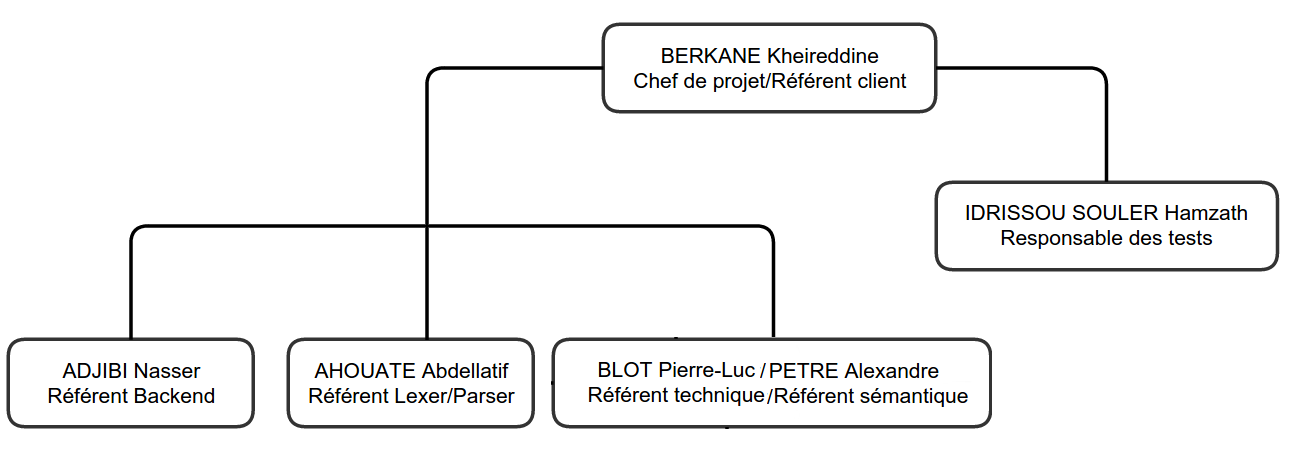
\includegraphics[width=7cm]{img/organigram.png}
          \caption{Organisation de l'équipe.}
          \label{organisaiton_de_l_equipe}
        \end{figure}      
      \end{block}
    \end{frame}

    \begin{frame}{Introduction}{Description du projet}
      \begin{block}{Description du projet}
        \begin{itemize}
          \item<1-> Objectif du compilateur LLVM: compiler en code natif le langage jouet kawa 
          \item<2-> Après le premier audit : mode de compilation monolithique 
          \item<3-> Notions supportées par Kawa : héritage, polymorphisme …
        \end{itemize}
      \end{block}
    \end{frame}
%%%%%%%%%%%%%%%%

\section{Architecture Globale}
    \begin{frame}{Architecture Globale}
      
        \begin{figure}[!h]
            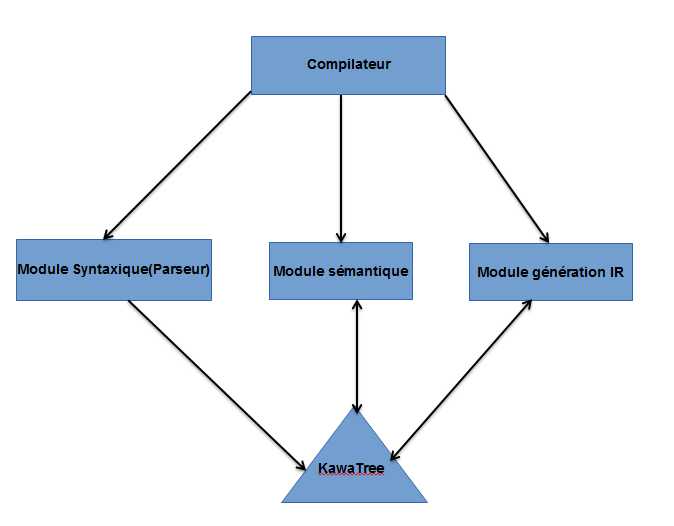
\includegraphics[width=7cm]{img/archi.PNG}
            \caption{Diagramme de l'architecture globale.}
            \label{diagramme_de_l_architecture_globale}
        \end{figure}      
      
    \end{frame}

  \subsection{Vue logique : KawaTree}
    \begin{frame}{Vue logique : KawaTree}
      \begin{figure}[!h]
          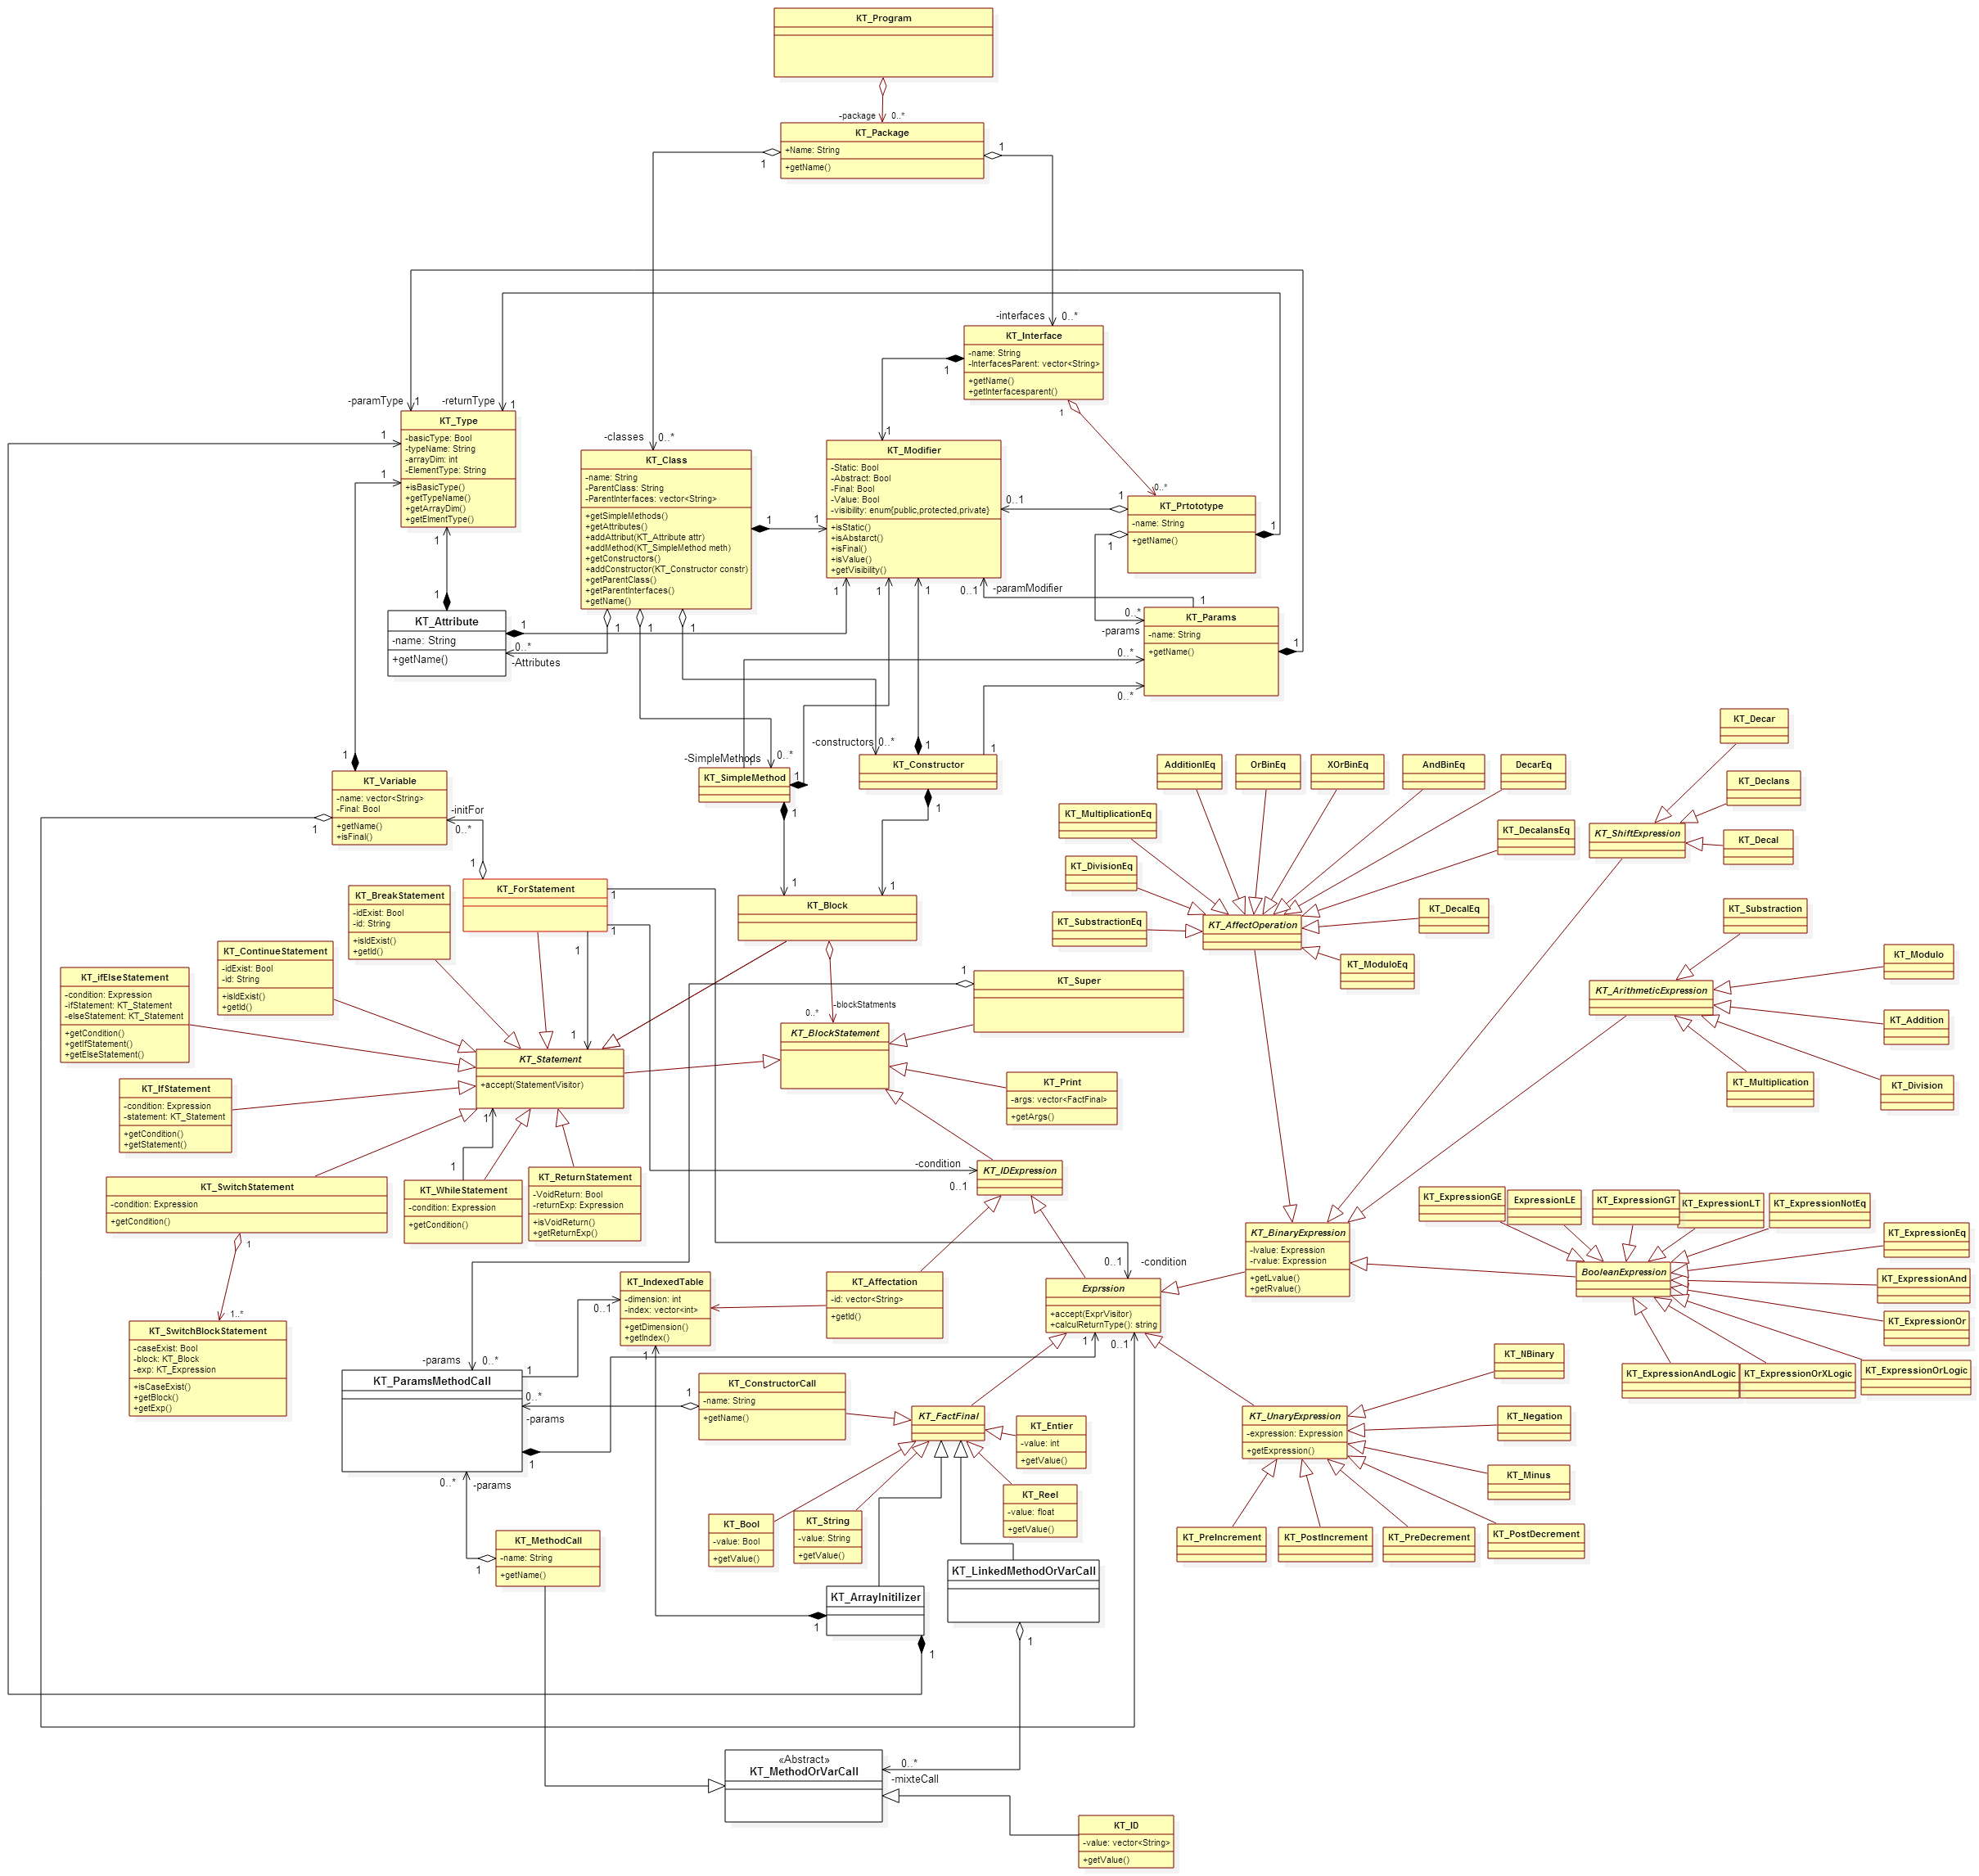
\includegraphics[width=7cm]{img/Diagramme_KT_V3_1.png}
          \caption{Diagramme de classe.}
          \label{diagramme_de_classe}
        \end{figure}
    \end{frame}
    
%%%%%%%%%%%%%%%%
\section{Bilan: syntaxique}
    \begin{frame}{Bilan: syntaxique}{Réalisation du module syntaxique}
    	
	      \begin{itemize}
	      	\item<1-> Objectif de Flex.
			\item<2-> Objectif de Bison.
			\item<3-> Le produit final de l'analyse syntaxique ?
			\item<4-> La couverture de la grammaire ?
	      \end{itemize}
    	
    \end{frame}

    \begin{frame}{Bilan: syntaxique}
    	
	      \begin{itemize}
	      	\item<1-> Analyse lexicale : mots clés, idfs …
			\item<2-> Analyse syntaxique :
			\begin{itemize}
				\item<3-> Implémentation de kawaTree
				\item<4-> Réalisation de la grammaire qui reconnait le langage kawa
				\item<5-> Réalisation du parseur pour monter l’information (respecte la STB)
			\end{itemize}
	      \end{itemize}
    	
    \end{frame}

    \begin{frame}{Bilan: syntaxique}{Problèmes rencontrés dans le module syntaxique}
    	
	      \begin{itemize}
	      	\item<1-> La complexité du langage Bison
			\item<2-> L’incompatibilité de l’ancienne architecture proposée.
	      \end{itemize}
    	
    \end{frame}

  
    
%%%%%%%%%%%%%%%%
\section{Bilan: sémantique}
    \begin{frame}{Bilan: sémantique}
    	\begin{block}{Pris en charge}
    		\begin{itemize}
				\item<1-> Des packages
				\item<2-> Des classes, des interfaces
				\item<3-> Des méthodes 
				\item<4-> Polymorphisme
				\item<5-> Héritage
    		\end{itemize}
    	\end{block}
    \end{frame}

    \begin{frame}{Bilan: sémantique}
    	\begin{block}{Non pris en charge}
    		\begin{itemize}
				\item<1-> Corps des méthodes/ sauf print
				\item<2-> Attributs
    		\end{itemize}
    	\end{block}

    \end{frame}
    \subsection{Les difficultés rencontrées}
	    \begin{frame}{Les difficultés rencontrées}{L'équipe}
	    	\begin{block}{Les difficultés rencontrées- L'équipe}
	    		\begin{itemize}
					\item<1-> Abandon d’un membre du groupe 
					\item<2-> Chef de projet contraint de délégué la tache par soucis personnel
					\item<3-> Membre absent durant une période critique
					\item<4-> Des conflits
	    		\end{itemize}
	    	\end{block}
	    \end{frame}

	    \begin{frame}{Les difficultés rencontrées}{Le projet et sa gestion}
	    	\begin{block}{Les difficultés rencontrées- Le projet et sa gestion}
	    		\begin{itemize}
					\item<1-> Un projet difficile à appréhender et à prendre en main
					\item<2-> Documents difficile à écrire à cause de cette complexité du projet
					\item<3-> Un langage non maîtrisé
					\item<4-> API LLVM inconnu et aucun référent 
	    		\end{itemize}
	    	\end{block}
	    \end{frame}

	\subsection{Erreurs commises}
	    \begin{frame}{Erreurs commises}{L'équipe}
	    	\begin{block}{Erreurs commises- L'équipe}
	    		\begin{itemize}
					\item<1-> Aucune recherche d’information concernant l’absence d’un membre
						\begin{itemize}
							\item<2-> Perte de temps pour remettre sur pieds un projet avec 1 personne de moins
						\end{itemize}
					\item<3-> Communication difficile
	    		\end{itemize}
	    	\end{block}
	    \end{frame}

	    \begin{frame}{Erreurs commises}{Le projet et sa gestion}
	    	\begin{block}{Erreurs commises- Le projet et sa gestion}
	    		\begin{itemize}
					\item<1-> Mauvaise évaluation des charges de travails (manque d’expérience)
					\item<2-> Des documents pas assez spécifiés, incomplets au lancement du projet
					\item<3-> Module géré par une personne seul
					\begin{itemize}
						\item<3-> Risque de SPLOF
					\end{itemize}
					\item<4-> Pas de mise en place itérative pour atteindre les objectifs
					\begin{itemize}
						\item<4-> Mauvaise gestion
					\end{itemize}

					\item<5-> des étapes, des jalons, des sous jalons
					\item<6-> PDD non respecté et pas de mise à jour
					\item<7-> PDD pas assez explicatif et ni détaillé
					\item<8-> Intégration
	    		\end{itemize}
	    	\end{block}
	    \end{frame}

	\subsection{Résumé}
		\begin{frame}{Difficultés rencontrées}{Résumé}
		    	\begin{block}{Difficultés rencontrées- Résumé}
		    		\begin{itemize}
						\item<1-> Difficultés rencontrés
						\item<2-> Abandon d’un membre du groupe 
						\item<3-> Chef de projet contraint de délégué la tache pour soucis personnel
						\item<4-> Des conflits
						\item<5-> Un projet difficile à appréhender et à prendre en main
						\item<6-> Documents difficile à écrire à cause de cette complexité du projet
						\item<7-> Un langage non maîtrisé
		    		\end{itemize}
		    	\end{block}
		\end{frame}

		\begin{frame}{Erreurs commises}{Résumé}
	    	\begin{block}{Erreurs commises- Résumé}
	    		\begin{itemize}
					\item<1-> Erreurs commises 
					\item<2-> Aucune recherche d’information
					\item<3-> Communication difficile
					\item<4-> PDD non respecté 
					\item<5-> Pas de gestion itérative pour atteindre l’objectif
					\item<6-> Documents trop peu spécifiés, incomplets
					\item<7-> Modules géré par une seule personne
	    		\end{itemize}
	    	\end{block}
	    \end{frame}

	    \begin{frame}{Problèmes}{Résumé}
	    	\begin{block}{Problèmes- Résumé}
	    		\begin{itemize}
					\item<1-> Retards à tous les niveaux
					\begin{itemize}
						\item<2-> Echecs des livraisons
						\item<3-> Remise en place d’un PDD
						\item<4-> Raccourcissement du projet
						\item<5-> Projet non terminé
					\end{itemize}
					\item<6-> Stress
					\item<7-> Tensions
	    		\end{itemize}
	    	\end{block}
	    \end{frame}

	\subsection{Expériences et acquis}
	    \begin{frame}{Expériences et acquis}{Sur la gestion de projet}
	    	\begin{block}{Expériences et acquis sur la gestion de projet}
	    		\begin{itemize}
	    			\item<1-> Documents essentiels pour une avancée commune dans la même direction malgré un travaille parallèle de chacun
					
					\item<2-> Mise en place d'un PDD détaillé, précis, et surveillé essentiel à une bonne avancée
					\item<3-> Mise en place de Test rapidement 
					\item<4-> Communiquer et partager le plus souvent possible
	    		\end{itemize}
	    	\end{block}
	    \end{frame}

	    \begin{frame}{Expériences et acquis}
	    	\begin{block}{Expériences et acquis}
	    		\begin{itemize}
					\item<1-> Outils collaboratifs
					\begin{itemize}
						\item<2-> Git : Partage de code 
						\item<3-> Slack : Plateforme de communication
					\end{itemize}
					\item<4-> Langages : c++
					\item<5-> Compréhension de la structure d’un compilateur

	    		\end{itemize}
	    	\end{block}
	    \end{frame}

	\subsection{Si c'était à refaire}

	    \begin{frame}{Ce qu’il faut changer}
	    	\begin{block}{Ce qu’il faut changer}
	    		\begin{itemize}
	    			\item<1-> Mieux aborder la création et la mise en place des documents dès le début
					\item<2-> Mettre en place un PDD plus précis et faire des points réguliers (tunnel, blocage, …) 
					\item<3-> Meilleur gestion des risques 
					\item<4-> Planification des tests
					\item<5-> Communication au sein de l’équipe

	    		\end{itemize}
	    	\end{block}
	    \end{frame}

	    \begin{frame}{Ce qu’il faut conserver}
	    	\begin{block}{Ce qu’il faut conserver}
	    		\begin{itemize}
	    			\item<1-> Echanges réguliers avec le client
					\item<2-> Réunions hebdomadaires
					\item<3-> Volonté de travail et d’efforts de chacun
	    		\end{itemize}
	    	\end{block}
	    \end{frame}
\section{Bilan: backend}
    \begin{frame}{Bilan: backend}{Le composant BackEnd}
    	\begin{block}{Le composant BackEnd}
	    	\begin{itemize}
				\item<1-> Rappel de la fonction du composant
				\begin{itemize}
					\item<2-> Interpreter le kawatree bien formé par la semantique en un code llvm ir.
				  	\item<3-> Produire le fichier \{nomp\_programme\}.ll
				  	\item<4-> Compiler le programme en un executable
				\end{itemize}
	    	\end{itemize}
	    \end{block}
	\end{frame}
	\begin{frame}{Bilan: backend}{Le composant BackEnd}
    	\begin{block}{Le composant BackEnd}
	    	\begin{itemize}

				\item<1-> Structure du Back
				 \begin{itemize}
				 	\item<2-> IRCompiler : composant parcourant le kawaTree
				  	\item<3-> Famille de generation : famille de composants metiers generant le code
				  	\item<4-> compilateur llc et gcc pour la compilation finale
				 	
				 \end{itemize}
	    	\end{itemize}
	    \end{block}
    \end{frame}

    \begin{frame}{Bilan: backend}{Deroulement de la mise en oeuvre du back-end}
    	\begin{block}{Deroulement de la mise en oeuvre du back-end}
	    	\begin{itemize}
				\item<1-> Phase d'etude de l'architecture llvm au cours de laquelle il fallait se familiarisé avec l'Api

				\item<2-> Etablissement de l'architecture du backend
					\begin{itemize}
						\item<3-> Famille de generation
						\item<4-> IRCompiler
					\end{itemize}

				\item<5-> Choix du mode de devellopement
					\begin{itemize}
						\item<6-> Le devellopement du back end etait ascendant dans la mesure ou j'ai commencé par a develloper la famille de generation avant puis essayer de les integrer progressivement au IRCompiler.
					\end{itemize}

	    	\end{itemize}
	    \end{block}
    \end{frame}

    \begin{frame}{Bilan: backend}{Deroulement de la mise en oeuvre du back-end}
    	\begin{block}{Deroulement de la mise en oeuvre du back-end}
	    	\begin{itemize}
				\item<1-> Probleme rencontré
				\begin{itemize}
					\item<2-> Révision à plusieurs reprise de l'architecture du back End à cause d'incoherences rencontrées au fur et a mesure que je devellopais, causant des retards

					\item<3-> Tests unitaires longs a mettre en oeuvre et une compilation lente, accruant la fatigue.

					\item<4-> Difficulté à tester le composant à cause d'une indisponibilité des tests. Causer par un manque de communication avec le testeur.

					\item<5-> Peu de reference pour le produire le code.
					
				\end{itemize}

	    	\end{itemize}
	    \end{block}
    \end{frame}

    \begin{frame}{Bilan: backend}{Deroulement de la mise en oeuvre du back-end}
    	\begin{block}{Deroulement de la mise en oeuvre du back-end}
	    	\begin{itemize}
	    		\item<1-> Erreur commise
	    		\begin{itemize}
					\item<2-> Sous estimation de la tache.
					\item<3-> Architecture defectuese.
					\item<4-> Sous estimation de l'importance des tests
	    		\end{itemize}
	    	\end{itemize}
	    \end{block}
    \end{frame}


    \begin{frame}{Bilan: backend}{Bilan}
    	\begin{block}{Bilan}
	    	\begin{itemize}
	    		\item<1-> Prise en charge de 
	    		\begin{itemize}
					\item<2-> Generation classe
					\item<3-> Generation methodes
					\item<4-> Generation appel de methodes
					\item<5-> Generation attributs
					\item<6-> Generation appel d'attribut
					\item<7-> Generation affectaion
					\item<8-> Generation affichage de types primitifs sur la sortie standards
					\item<9-> Generation prise Table adHoc
	    			
	    		\end{itemize}
	    	\end{itemize}
	    \end{block}
	\end{frame}

	\begin{frame}{Bilan: backend}{Bilan}
    	\begin{block}{Bilan}
    		\begin{itemize}
				\item<1-> Prise en charge mais non integrer
				\begin{itemize}
					\item<2-> Operation binaires
				\end{itemize}

				\item<3-> Non pris en charge
				\begin{itemize}
					\item<4-> Bloc intrucion a plusieurs niveau
				\end{itemize}

				\item<5-> Documentation pas en sync avec l'implementation.
	    	\end{itemize}
	    \end{block}
    \end{frame}

    \begin{frame}{Bilan: backend}{Si c'était à refaire}
    	\begin{block}{Si c'était à refaire}
	    	\begin{itemize}
	    		\item<1-> Meilleur communication avec le testeur
				\item<2-> Revoir l'architecture
				\item<3-> Changer le mode de dev
	    	\end{itemize}
	    \end{block}
    \end{frame}

	\begin{frame}{Bilan: backend}{Demo}
    	\begin{itemize}
    		\item<1-> Conclure avec la presentation d'une demo du back end
    	\end{itemize}
    \end{frame}


\section{Test}
    \begin{frame}{Test}    	
		\begin{itemize}
			\item Pourquoi des Tests?
		\end{itemize}
	
    \end{frame}

    \subsection{Stratégie des Tests}
	\begin{frame}{Stratégie des Tests}{Pour valider les procédures de tests}
		\begin{block}{Pour valider les procédures de tests}
			\begin{enumerate}
				\item<1-> Tests Unitaires.
				\item<2-> Tests d'intégrations.
				\item<3-> Tests de non regressions.
			\end{enumerate} 
			\pause
			\pause
			\pause
			
		\end{block}
		\begin{block}{NB :} % Bloc normal
			A chaque fois qu’un test est réalisé il fallait notifier\\
		    le résultat obtenu dans le tableau des procédures\\
           (se trouvant dans le cahier de recette).
            L’objectif étant d’avoir tous les tests validé à la fin du projet.\\
         	Et que ces tests touchent le plus de ligne de code possible; \\
        	 c’est ce qu’on appelle la couverture de code. 
		\end{block}
	\end{frame}

	\subsection{Bilan Tests}
		\begin{frame}{Bilan Tests}{Différents Modules}
			\begin{enumerate}
				\item<1-> Module Syntaxique.
				\item<2-> Module Sémantique.
				\item<3-> Structure KawaTree.
			\end{enumerate} 		
		\end{frame}

	%Gestion des Anomalies
	\subsection{Gestion des Anomalies}
		
		\begin{frame}{Gestion des Anomalies}{Echec Test}
			\begin{block}{Que doit on faire?}
				\begin{itemize}
					\item<1-> Echec d'un test.
					\item<2-> Résolution du problème.
					\item<3-> Validation de la résolution du problème
				\end{itemize} 
			\end{block}
		\end{frame}

	%Automatisation des Tests
	\subsection{Automatisation des tests}
		\begin{frame}{Automatisation}{Difficultés rencontrées}
			\begin{itemize}
				\item<1-> Prise en main de CppUnit.
			\end{itemize} 
		\end{frame}


\section{Bilan: projet}
    \begin{frame}{Bilan: projet}
    	
    \end{frame}


%%%%%%%%%%%%%%%%

{\aauwavesbg
\begin{frame}[plain,noframenumbering]
  \finalpage{Merci pour votre attention !\\
  Avez-vous des questions ?
  }
\end{frame}}
%%%%%%%%%%%%%%%%

\end{document}
